\part{Bosonic path integrals}

\chapter{Introduction}

    In this chapter, we will review some notions of quantum mechanics: probability amplitude of the two-slits experiment and first (canonical) quantisation.

\section{Two slit experiment}

    In quantum mechanics, there are two equivalent methods to quantise: operator formalism and path integrals. The latter has been introduced by Feynman and is useful for two reasons: quantisation of (non-abelian) gauge theories in the standard model and relation between quantum field theory and statistical mechanics.

    In order to introduce the concept of path integral, we show the two slits experiment. Consider an electron, created by a source, that passes through a barrier with two slits and reach a detector screen, forming a figure of interference. See Figure~\eqref{fig:b:slits}. 
    
    \begin{figure}[h!]
        \centering
        \begin{tikzpicture}
                
        \draw[] (2.5,0) -- (2.5,1) node[xshift=-0.4cm, yshift=-0.2cm] {$c_1$};
        \draw[] (2.5,1.5) -- (2.5,2.5) node[xshift=-0.4cm, yshift=0.6cm] {$c_2$};
        \draw[] (2.5,3) -- (2.5,4) ;
        \draw[] (5,0) -- (5,4) ;

        \draw[] (5,4) to[bend left=50] (5, 3.5) to[bend left=60] (5,2.5) to[bend left=50] (5.5, 2) to[bend left=50] (5, 1.5) to[bend left=60] (5, 0.5) to[bend left=50] (5,0);

        \filldraw[black] (0,2) circle (0.05) node[below left] {source};

        \draw[] (0,2) -- (2.5,1.25);
        \draw[] (0,2) -- (2.5,2.75);
        \draw[] (2.5,1.25) -- (5,3);
        \draw[] (2.5,2.75) -- (5,3);

        \end{tikzpicture}
        \caption{Two slits experiment with figure of interference on the screen and two possible paths $c_1$ and $c_2$ for the electron.}
        \label{fig:b:slits}
    \end{figure}
    
    The standard way to study such system is to highlight the wave behaviour of the electron and calculate the interference pattern with the Huygens principle. However, Feynman proposed an alternative way. The electron is a particle which manage to travel all the possible paths from the source to the screen. Therefore, for each path $c_i$, we can associate an amplitude $A (c_i)$ and the total amplitude $A_{tot} = \sum_i A(c_i)$ is related to the probability to find the particle in a point of the detector screen $p = |A_{tot}|^2$. This probability has unit norm and a phase equal to $\frac{S}{\hbar}$, where $S$ is the action of the particle:
    \begin{equation*}
        A(c_i) = \exp( \frac{i}{\hbar}) S(c_i) ~,
    \end{equation*}
    and the total amplitude is 
    \begin{equation*}
        A_{tot} = \sum_i \exp( \frac{i}{\hbar}) S(c_i) ~.
    \end{equation*}

    \begin{figure}[h!]
        \centering
        \begin{tikzpicture}
                
        \draw[] (2.5,0) -- (2.5,1) node[xshift=-0.4cm, yshift=-0.2cm] {$c_1$};
        \draw[] (2.5,1.5) -- (2.5,2.5) node[xshift=-0.4cm, yshift=0.6cm] {$c_2$};
        \draw[] (2.5,3) -- (2.5,4) ;
        \draw[] (5,0) -- (5,4) ;

        \filldraw[black] (0,2) circle (0.05) node[below left] {source};

        \draw[] (0,2) -- (2.5,1.25);
        \draw[] (0,2) -- (2.5,2.75);
        \draw[] (2.5,1.25) -- (5,3) node[xshift=-1cm, yshift=0.3cm] {$D$};
        \draw[] (2.5,2.75) -- (5,3) node[xshift=-0.8cm, yshift=-1.1cm] {$D$};
        \draw[] (2.5,2.75) -- (3.3, 1.8) node[xshift=-0.2cm, yshift=-0.5cm] {$d$};

        \end{tikzpicture}
        \caption{Two slits experiment with distances $d \ll D$.}
        \label{fig:b:slits2}
    \end{figure}

    Now, consider the simple case in which the electron is treated as  a free particle with associated action 
    \begin{equation*}
        S[q] = \int_0^T dt ~ \frac{m}{2} \dot q^2 ~.
    \end{equation*}
    We suppose also that the difference between the two path is $d \ll D$, see Figure~\ref{fig:b:slits2}, so that we evaluate the action for the path $c_1$ 
    \begin{equation*}
        S(c_1) = \frac{m}{2} \frac{D^2}{T^2} T = \frac{m}{2} \frac{D^2}{T}
    \end{equation*}
    and for the path $c_2$ 
    \begin{equation*}
    \begin{aligned}
        S(c_2) & = \frac{m}{2} \frac{(D+d)^2}{T^2} T = \frac{m}{2T} (D^2 + 2 D d + O(d^2)) \\ & = \frac{m}{2} \frac{D^2}{T} + \frac{m D d}{T} O(d^2) = \frac{m}{2} \frac{D^2}{T} + pd + O(d^2) = S(c_1) + pd + O(d^2) ~,
    \end{aligned}
    \end{equation*}
    where we roughly estimate $p \sim \frac{m D}{T}$. Therefore, the total amplitude is 
    \begin{equation*}
        A_{tot} = A(c_1) + A(c_2) = \exp (\frac{i}{\hbar} S(c_1)) + \exp (\frac{i}{\hbar} S(c_2)) = \exp (\frac{i}{\hbar} S(c_1)) \Big (1 + \exp (\frac{i}{\hbar} pd) \Big) + O(d^2) ~. 
    \end{equation*}
    Notice that the maximum probability is given when 
    \begin{equation*}
        \exp(\frac{i}{\hbar} pd) = 1 \quad \Rightarrow \quad \frac{pd}{\hbar} = 2 \pi n ~,
    \end{equation*}
    where $n \in \mathbb Z$. We recover quantum mechanics, since we recognise the Compton wavelength of the electron
    \begin{equation*}
        \lambda = \frac{\hbar}{p} ~,
    \end{equation*}
    and we find the relation 
    \begin{equation*}
        \frac{d}{\lambda} = n ~.
    \end{equation*}

    We can generalise by increasing the number of slits and intermediary screens to have all the possible paths between the initial point (source) and the final point (detector). The action becomes 
    \begin{equation*}
        S[q] = \int_{t_i}^{t_f} dt ~L(q, \dot q) 
    \end{equation*}
    and the transition amplitude in the continuum limit becomes
    \begin{equation*}
        A = \sum_i \exp(\frac{i}{\hbar} S(c_i)) = \int \mathcal D q ~ \exp (\frac{i}{\hbar} S[q]) ~,
    \end{equation*}
    where $S[q]$ is a functional, $A$ is an integral functional and $\mathcal D q$ is the measure in the path space.

    We can recover the classical limit by noticing that, for macroscopic systems, the rate $\frac{S}{\hbar}$ is very big and small variations $\frac{\delta S}{\hbar}$ are bigger than $i \pi$. Therefore, the amplitudes of nearby paths cancel by destructive interference, unless it is the real classical path, since $\delta S = 0$. This happens because for macroscopic systems, the action is so big that can reach any value and its opposite, so that they cancel each other.

\section{Transition amplitude}

    It is useful to recall the procedure of canonical quantisation and how transition amplitudes come up. Given an Hamiltonian classical system, canonical quantisation consists in promoting phase space coordinates (generalised coordinates and momenta) into linear operators acting on a Hilbert space, satisfying the commutator relations 
    \begin{equation*}
        [\hat x^i, \hat p_j] = i \hbar \delta^i_j ~, \quad [\hat x^i, \hat x^j] = [\hat p^i, \hat p^j] = 0 ~,
    \end{equation*}
    which are obtained by the Poisson brackets in the following way
    \begin{equation*}
        [ ~ , ~ ] = i \hbar \{~ , ~\}_{PB} ~.
    \end{equation*}
    All observables are linear self-adjoint operators acting on the Hilbert space. A special role plays the Hamiltonian of the system, since it governs time evolution via the Schroedinger equation 
    \begin{equation*}
        i \hbar \pdv{}{t} \ket{\psi} = \hat H \ket{\psi} ~.
    \end{equation*} 
    It becomes operative once an irreducible unitary representation of the algebra of commutators has been found, since by the Stone-Von Neumann theorem states that they are all equivalent. The latter theorem show also that Schroesinger (states evolve, operators not) and Heisenberg (operators evolve, states not) pictures are equivalent.

    Now, consider a $1$-dimensional particle in the presence of a potential $V(x)$, such that its action in configuration space is 
    \begin{equation*}
        S[x(t)] = \int dt ~ \Big ( \frac{m}{2} \dot x^2 - V(x) \Big) ~. 
    \end{equation*}
    The conjugate momentum is defined as 
    \begin{equation*}
        p = \pdv{L}{\dot x} = m \dot x ~.
    \end{equation*}
    By a Legendre transformation, we can introduce the Hamiltonian 
    \begin{equation*}
        H = p \dot x - L = p \frac{p}{m} + \frac{p^2}{2m} + V(x) = \frac{p^2}{2m} ~.
    \end{equation*}
    Therefore, the Hamiltonian action in phase space becomes
    \begin{equation*}
        S[x(t)] = \int dt ~ \Big (p \dot x - H) = \int dt ~ \Big ( p \dot x - \frac{p^2}{2m} - V(x)) ~. 
    \end{equation*}
    The Poisson brackets between coordinate and momentum are 
    \begin{equation*}
        \{x,x\}_{PB} = \{p,p\}_{PB} = 0 ~, \quad \{x,p\}_{PB} = 1 ~.
    \end{equation*}
    By means of the canonical quantisation, we find the canonical commutation relations 
    \begin{equation*}
        [\hat x, \hat x] = [\hat p, \hat p] = 0 ~, \quad [\hat x, \hat p] = i \hbar ~.
    \end{equation*}
    The Hamiltonian is also promoted to an operator
    \begin{equation*}
        \hat H = \frac{1}{2m} \hat p^2 + V(\hat x) ~.
    \end{equation*}
    Working in coordinate representation, the eigenstates of the position are 
    \begin{equation*}
        \hat x \ket{x} = x \ket{x} ~,
    \end{equation*}
    such that they satisfy 
    \begin{equation*}
        \braket{x}{x'} = \delta (x - x') ~, \quad \mathbb I = \int dx ~ \ket{x} \bra{x} ~.
    \end{equation*}
    The momentum operator in this representation is 
    \begin{equation*}
        \hat p = - i \hbar \pdv{}{x} ~.
    \end{equation*}
    Hence, the Schroedinger equation reads as
    \begin{equation*}
        i \hbar \pdv{}{t} \psi(t,x) = \Big (\frac{1}{2m} \hat p^2 + V(\hat x) \Big ) \psi(t,x) = \Big (-\frac{\hbar^2}{2m} \pdvdu{}{x} + V(x) \Big) \psi(t,x) ~.
    \end{equation*}

    It is possible to formulate time evolution in a different way: for any time-independent Hamiltonian, we can solve the Schroedinger equation introducing an evolution operator 
    \begin{equation*}
        \ket{\psi(t)} = \exp(- \frac{i}{\hbar} \hat H t) \ket{\psi (t_0)} ~,
    \end{equation*}
    where $t_0$ is the initial time and $t$ is a generic final time.
    \begin{proof}
        In fact, 
        \begin{equation*}
            i \hbar \pdv{}{t} \ket{\psi(t)} = i \hbar \pdv{}{t} \exp(- \frac{i}{\hbar} \hat H t) \ket{\psi (t_0)} = i \hbar \Big ( - \frac{i}{\hbar} \hat H \Big ) \exp(- \frac{i}{\hbar} \hat H t) \ket{\psi (t_0)} = \hat H \ket{\psi(t)} ~. 
        \end{equation*}
    \end{proof}
    Hence, the transition amplitude to find the system from the initial state $\psi_0$ to the final state $\psi_f$ after a time $T = t_f - t_0$ is obtained by projecting the solution for time $T$ onto the final state 
    \begin{equation*}
        \braket{\psi (t_f)}{\psi(T)} = \bra{\psi (t_f)} \exp(- \frac{i}{\hbar} \hat H T) \ket{\psi (t_0)} ~,
    \end{equation*}
    which can be rewritten in coordinate representation is 
    \begin{equation*}
        A (x_0, x_f, T) = \bra{x_f} \exp(- \frac{i}{\hbar} \hat H T) \ket{x_0} ~.
    \end{equation*}
    Notice that it is a matrix element between position eigenstates of the evolution operator.
    \begin{proof}
        In fact, 
        \begin{equation*}
        \begin{aligned}
            \braket{\psi_f}{\psi(T)} & = \bra{\psi_f} \exp(- \frac{i}{\hbar} \hat H T) \ket{\psi_0} = \bra{\psi_f} \mathbb I \exp(- \frac{i}{\hbar} \hat H T) \mathbb I \ket{\psi_0} \\ & = \int dx_f ~ \underbrace{\braket{\psi_f}{x_0}}_{\psi_f(x_f)} \bra{x_0} \exp(- \frac{i}{\hbar} \hat H T) \int dx_0 ~ \ket{x_0} \underbrace{\braket{x_i}{\psi_0}}_{\psi_i(x_0)} \\ & = \int dx_0 \int dx_f ~ \psi_f^* (x_f) \psi_0 (x_0) \bra{x_f} \exp(- \frac{i}{\hbar} \hat H T) \ket{x_0} \\ & = \int dx_0 \int dx_f ~ \psi_f^* (x_f) \psi_0 (x_0) A (x_0, x_f, T) ~,
        \end{aligned}
        \end{equation*}
        where we have used the completeness relation 
        \begin{equation*}
            \mathbb I = \int dx ~ \ket{x} \bra{x} ~.
        \end{equation*}
    \end{proof}
    Notice that it satisfies the Schroedinger equation 
    \begin{equation*}
        i \hbar \pdv{}{T} A (x_0, x_f, T) = \hat H A (x_0, x_f, T) ~,
    \end{equation*}
    with initial conditions
    \begin{equation*}
        A (x_0, x_f, 0) = \delta (x_f - x_0) ~.
    \end{equation*}
    \begin{proof}
        In fact,
        \begin{equation*}
        \begin{aligned}
            i \hbar \pdv{}{T} A (x_0, x_f, T) & = i \hbar \pdv{}{T} \bra{x_f} \exp(- \frac{i}{\hbar} \hat H T) \ket{x_0} \\ & = i \hbar \Big (- \frac{i}{\hbar} \hat H \Big) \bra{x_f} \exp(- \frac{i}{\hbar} \hat H T) \ket{x_0}  \\ & =  \hat H \bra{x_f} \exp(- \frac{i}{\hbar} \hat H T) \ket{x_0} = \hat H  A (x_0, x_f, T) ~.
        \end{aligned}
        \end{equation*}
    \end{proof}

\chapter{Path integrals and more}

    In this chapter, we will introduce path integral in phase space and then after an integration in the configuration space. Furthermore, we will study its connection with statistical mechanics with the Wick rotation and some useful tools: correlation functions, Gaussian integrals and hypercondensed notation.

\section{Path integrals in phase and configuration space}

    The path integral in phase space is 
    \begin{equation*}
    \begin{aligned}
        A & = \lim_{N \rightarrow \infty} \int \Big (\prod_{k=1}^{N-1} d x_k \Big ) \Big (\prod_{k=1}^{N} \frac{d p_k}{2\pi \hbar} \Big ) \exp(\frac{i \epsilon}{\hbar} \sum_{k=1}^{N} \Big (p_k \frac{x_k - x_{k-1}}{\epsilon} - H(x_{k-1}, p_k))) \\ & = \int \mathcal D x ~ \mathcal D p ~ \exp(\frac{i}{\hbar} S[x,p]) ~,
    \end{aligned}
    \end{equation*}
    where $\epsilon =\frac{T}{N} $.

    \begin{proof}
        We split the transition amplitude into the product of $N$ factors, by putting $N-1$ coordinate completeness relations
        \begin{equation*}
        \begin{aligned}
            A (x_0, x_f, T) & = \bra{x_f} \exp(- \frac{i}{\hbar} \hat H T) \ket{x_0} = \bra{x_f} \exp(- \frac{i}{\hbar} \hat H \underbrace{\frac{T}{N}}_\epsilon N) \ket{x_i} \\ & = \bra{x_f} \exp(- \frac{i}{\hbar} \hat H \epsilon)^N \ket{x_0} = \bra{x_f} \underbrace{\exp(- \frac{i}{\hbar} \hat H \epsilon) \mathbb I \ldots \mathbb I \exp(- \frac{i}{\hbar} \hat H \epsilon)}_{\text{N exp and N - 1 identities}} \ket{x_0} \\ & = \int \Big ( \prod_{k=1}^{N-1} dx_k \Big) \Big ( \prod_{k=1}^{N} \bra{x_k} \exp(- \frac{i}{\hbar} \hat H \epsilon) \ket{x_{k-1}} \Big) ~,
        \end{aligned}
        \end{equation*}
        where $x_{k=1} = x_0$ and $x_{k=N} = x_f$. 
        Now, we insert a momentum completeness relation 
        \begin{equation*}
        \begin{aligned}
            & = \int \Big ( \prod_{k=1}^{N-1} dx_k \Big) \Big ( \prod_{k=1}^{N} \bra{x_k} \mathbb I \exp(- \frac{i}{\hbar} \hat H \epsilon) \ket{x_{k-1}} \Big) \\ & = \int \Big ( \prod_{k=1}^{N-1} dx_k \Big) \Big ( \prod_{k=1}^{N} \frac{dp_k}{2 \pi \hbar} \Big) \prod_{k=1}^{N}\underbrace{\braket{x_k}{p_k}}_{\exp(\frac{i}{\hbar} p_k x_k)} \bra{p_k} \exp(- \frac{i}{\hbar} \hat H \epsilon) \ket{x_{k-1}} \\ & = \int \Big ( \prod_{k=1}^{N-1} dx_k \Big) \Big ( \prod_{k=1}^{N} \frac{dp_k}{2 \pi \hbar} \Big) \prod_{k=1}^{N} \exp(\frac{i}{\hbar} p_k x_k) \bra{p_k} \exp(- \frac{i}{\hbar} \hat H \epsilon) \ket{x_{k-1}} ~.
        \end{aligned}
        \end{equation*}
        Notice that there is integration over $N-1$ coordinates and $N$ momenta because we are working in coordinate representation. So far, we compute the exact development. Now, we go infinitesimally with $N \gg 1$ or equivalently $\epsilon \ll 1$. First, we calculate 
        \begin{equation*}
        \begin{aligned}
            \bra{p_k} \exp(- \frac{i}{\hbar} \hat H(\hat x, \hat p) \epsilon) \ket{x_{k-1}} & = \bra{p_k} (1 - \frac{i}{\hbar} \hat H (\hat x, \hat p) \epsilon + \ldots) \ket{x_{k-1}} \\ & = \braket{p_k}{x_{k-1}} - \bra{p_k} \frac{i}{\hbar} \hat H (\hat x, \hat p) \epsilon \ket{x_{k-1}} + \ldots \\ & = \braket{p_k}{x_{k-1}} - \bra{p_k} \frac{i}{\hbar} \hat H (x_{k-1}, p_k) \epsilon \ket{x_{k-1}} + \ldots \\ & = \braket{p_k}{x_{k-1}} \exp(- \frac{i}{\hbar} H (x_{k-1}, p_k) \epsilon) ~,
        \end{aligned}
        \end{equation*}
        where we have used the fact that the Hamiltonian is a function of coordinates and momenta, therefore, they have the same eigenstates. Hence, we find
        \begin{equation*}
        \begin{aligned}
            & = \lim_{N \rightarrow \infty} \int \Big ( \prod_{k=1}^{N-1} dx_k \Big) \Big ( \prod_{k=1}^{N} \frac{dp_k}{2 \pi \hbar} \Big) \prod_{k=1}^{N} \exp(\frac{i}{\hbar} p_k x_k) \bra{p_k} \exp(- \frac{i}{\hbar} \hat H \epsilon) \ket{x_{k-1}} \\ & = \lim_{N \rightarrow \infty} \int \Big ( \prod_{k=1}^{N-1} dx_k \Big) \Big ( \prod_{k=1}^{N} \frac{dp_k}{2 \pi \hbar} \Big) \prod_{k=1}^{N} \exp(\frac{i}{\hbar} (p_k (x_k - x_{k-1}) - H(x_{k-1}, p_k) \epsilon )) \\ & = \lim_{N \rightarrow \infty} \int \Big ( \prod_{k=1}^{N-1} dx_k \Big) \Big ( \prod_{k=1}^{N} \frac{dp_k}{2 \pi \hbar} \Big) \prod_{k=1}^{N} \exp(\frac{i}{\hbar} \underbrace{\epsilon}_{dt} (\underbrace{p_k}_p \underbrace{\frac{x_k-x_{k-1}}{\epsilon}}_{\dot x} - \underbrace{H(x_{k-1}, p_k)}_{H} )) \\ & = \int \mathcal D x ~ \mathcal D p ~ \exp(\frac{i}{\hbar} S[x,p]) ~,
        \end{aligned}
        \end{equation*}
        where we the last passage is only a symbolic definition $\mathcal D x \mathcal D p$ and we have passed into the continuum limit with  
        \begin{equation*}
            \sum_{k=1}^N \epsilon (p_k \frac{x_k - x_{k-1}}{\epsilon} - H(x_{k-1}, p_k)) \quad \rightarrow \quad \int_{t_0}^{t_f} dt ~ (p \dot x - H(x, p)) ~,
        \end{equation*}
        \begin{equation*}
            x_k = x (t_0 + k \epsilon) ~, \quad p_k = p(t_0 + k \epsilon) \quad \rightarrow \quad x(t) ~, \quad p(t) ~.
        \end{equation*}
    \end{proof}

    The path integral in configuration space is 
    \begin{equation}\label{b:pathconfig}
    \begin{aligned}
        A & = \lim_{N \rightarrow \infty} \int \Big (\prod_{k=1}^{N-1} d x_k \Big ) \Big (\frac{m}{2 \pi i \hbar \epsilon} \Big )^{\frac{N}{2}} \exp(\frac{i \epsilon}{\hbar} \sum_{k=1}^{N} \Big (\frac{m}{2} \frac{(x_k - x_{k-1})^2}{\epsilon^2} - V(x_{k-1})\Big )) \\ & = \int \mathcal D x ~ \exp(\frac{i}{\hbar} S[x]) ~.
    \end{aligned}
    \end{equation}
    \begin{proof}
        With the use of the Gaussian integral, 
        \begin{equation*}
            \int_{- \infty}^\infty dp ~ \exp(- \frac{\alpha}{2} p^2 + \beta p) = \sqrt{\frac{2\pi}{\alpha}} \exp(\frac{\beta^2}{2\alpha}) ~,
        \end{equation*}
        which in our case $\alpha$ and $\beta$ are 
        \begin{equation*}
            \alpha = \frac{i\epsilon}{\hbar m} ~, \quad \beta = \frac{i}{\hbar} (x_k - x_{k-1}) ~,
        \end{equation*}
        we find 
        \begin{equation*}
        \begin{aligned}
            A & = \lim_{N \rightarrow \infty} \int \Big ( \prod_{k=1}^{N-1} dx_k \Big) \Big ( \prod_{k=1}^{N} \frac{dp_k}{2 \pi \hbar} \Big) \exp \Big ( \frac{i}{\hbar} \sum_{k=1}^N \epsilon (p_k \frac{x_k - x_{k-1}}{\epsilon} - \frac{p_k^2}{2m} - V(x_{k-1}) ) \Big ) \\ & = \lim_{N \rightarrow \infty} \int \Big (\prod_{k=1}^{N-1} d x_k \Big ) \Big (\frac{1}{2\pi\hbar} \Big (\frac{2\pi \hbar m}{i \epsilon} \Big)^{\frac{N}{2}} \Big ) \exp \Big ( \frac{i}{\hbar} \sum_{k=1}^N \epsilon (\frac{\hbar m}{2 i \epsilon} (\frac{i}{\hbar} (x_k - x_{k-1}))^2 - V(x_{k-1}) ) \Big ) \\ & = \lim_{N \rightarrow \infty} \int \Big (\prod_{k=1}^{N-1} d x_k \Big ) \Big (\frac{1}{2\pi\hbar} \Big (\frac{2\pi \hbar m}{i \epsilon} \Big)^{\frac{N}{2}}  \exp(\frac{i \epsilon}{\hbar} \sum_{k=1}^{N} \epsilon \Big (\frac{m (x_k - x_{k-1})^2}{\epsilon^2} - V(x_{k-1})) \Big ) \Big ) \\ & = \lim_{N \rightarrow \infty} \int \prod_{k=1}^{N-1} d x_k \Big (\frac{m}{2 \pi \hbar i \epsilon} \Big)^{\frac{N}{2}}  \exp(\frac{i \epsilon}{\hbar} \sum_{k=1}^{N} \epsilon \Big (\frac{m (x_k - x_{k-1})^2}{\epsilon^2} - V(x_{k-1})) \Big ) \\ & = \int \mathcal D x ~ \exp(\frac{i}{\hbar} S[x]) ~.
        \end{aligned}
        \end{equation*}
    \end{proof}
    Pictorially, the discretised and continuum path integral can be seen in Figure~\eqref{fig:b:path}.

    \begin{figure}[h!]
        \centering
        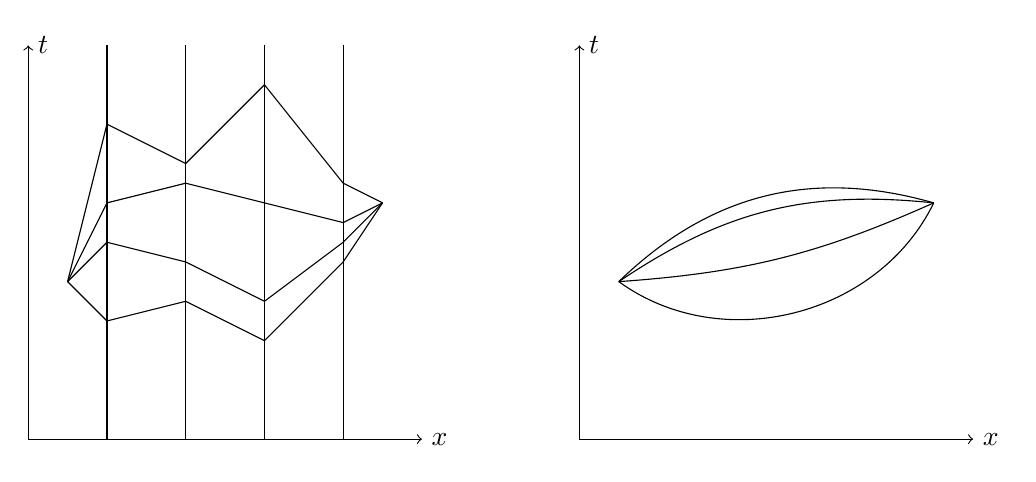
\begin{tikzpicture}
        \draw[->] (0,0) -- (5,0) node[right] {$x$};
        \draw[->] (0,0) -- (0,5) node[right] {$t$};

        \draw[->] (7,0) -- (12,0) node[right] {$x$};
        \draw[->] (7,0) -- (7,5) node[right] {$t$};

        \draw[] (1,0) -- (1,5);
        \draw[] (2,0) -- (2,5);
        \draw[] (3,0) -- (3,5);
        \draw[] (4,0) -- (4,5);

        \draw[] (0.5,2) -- (1,4); \draw[] (1,4) -- (2,3.5);
        \draw[] (2,3.5) -- (3,4.5); \draw[] (3,4.5) -- (4,3.25); 
        \draw[] (4,3.25) -- (4.5,3);  

        \draw[] (0.5,2) -- (1,3); \draw[] (1,3) -- (2,3.25);
        \draw[] (2,3.25) -- (3,3); \draw[] (3,3) -- (4,2.75); 
        \draw[] (4,2.75) -- (4.5,3);  

        \draw[] (0.5,2) -- (1,2.5); \draw[] (1,2.5) -- (2,2.25);
        \draw[] (2,2.25) -- (3,1.75); \draw[] (3,1.75) -- (4,2.5); 
        \draw[] (4,2.5) -- (4.5,3);  

        \draw[] (0.5,2) -- (1,1.5); \draw[] (1,1.5) -- (2,1.75);
        \draw[] (2,1.75) -- (3,1.25); \draw[] (3,1.25) -- (4,2.25); 
        \draw[] (4,2.25) -- (4.5,3);  
                
        \draw[] (7.5,2) to[bend right=10] (11.5,3);
        \draw[] (7.5,2) to[bend right=50] (11.5,3);
        \draw[] (7.5,2) to[bend left=20] (11.5,3);
        \draw[] (7.5,2) to[bend left=30] (11.5,3);

        \end{tikzpicture}
        \caption{Path integral in the discrete (left) and continuous (right) version.}
        \label{fig:b:path}
    \end{figure}

    \begin{example}
        Consider a free particle with $N = 1$, $T = \epsilon$ and $V(x) = 0$. Using~\eqref{b:pathconfig}, the path integral is 
        \begin{equation*}
            A = \sqrt{\frac{m}{2\pi\hbar i T}} \exp(\frac{i}{\hbar} \frac{m(x_f - x_i)^2}{2T}) ~.
        \end{equation*}
        The free particle is a very special case, because the semiclassical approximation with $N = 1$ is exact, so that we do not have to compute the limit $N \rightarrow \infty$. To compute the path integral, we formally use the continuum limit, in particular its property of translation invariance. Heuristically, the action is 
        \begin{equation*}
            S[x_{cl}] = \int_0^T \frac{m}{2} \frac{(x_f - x_i)^2}{T^2} = T \frac{m}{2} \frac{(x_f - x_i)^2}{T^2} =  \frac{m(x_f - x_i)^2}{2T} ~.
        \end{equation*}
        and a classical solution of the equation of motions is 
        \begin{equation*}
            x_{cl} (t) = x_i + \frac{x_f - x_i}{T} t ~.
        \end{equation*}
        We can add to a generic classical path, a quantum fluctuation $q(t)$
        \begin{equation*}
            x(t) = x_{cl}(t) + q(t) ~,
        \end{equation*}
        such that $q(0) = 0$ and $q(T) = 0$ to preserve boundary conditions. We can think of $x_{cl} (t)$ as the origin in the space of functions and compute the path integral
        \begin{equation*}
        \begin{aligned}
            A & = \int \mathcal D x \exp (\frac{i}{\hbar} S[x(t)]) = \int \mathcal D x \exp (\frac{i}{\hbar} S[x_{cl}(t) + q(t)]) \\ & = \int \mathcal D x \exp (\frac{i}{\hbar} S[x_{cl}(t)] + S [q(t)]) = \int \mathcal D x \exp (\frac{i}{\hbar} S[x_{cl}(t)]) \underbrace{\int \mathcal D x \exp (\frac{i}{\hbar} S [q(t)])}_N \\ & = N \exp(\frac{i}{\hbar} S[x_{cl}(t)]) = N \exp( \frac{i}{\hbar} \frac{m (x_f - x_0)^2 }{2 T} ) ~,
        \end{aligned}
        \end{equation*}
        where we have used the translation invariance $\mathcal D x = \mathcal D (x + q) = \mathcal D q$ and for the mixed term we have used the equations of motion $\ddot x = 0$ 
        \begin{equation*}
        \begin{aligned}
            S[x_{cl} + q] & = \frac{m}{2} \int dt ~ \dv{}{t} (x_{cl} + q)^2 =  \frac{m}{2} \int dt ~ \dv{}{t} (x_{cl} + q) \dv{}{t} (x_{cl} + q) \\ & = \frac{m}{2} \int dt ~ (\dot x_{cl} + \dot q )^2 = \frac{m}{2} \int dt ~ (\dot x_{cl}^2 + \dot q^2 + 2 \dot x_{cl} \dot q) \\ & = S[x_{cl}] + S[q] + m \int dt ~ \underbrace{\dot x_{cl} \dot q}_{- \ddot x_{cl} q + \text{boundary terms}} \\ & = S[x_{cl}] + S[q] - m \int dt ~ \underbrace{\ddot x_{cl}}_0 q = S[x_{cl}] + S[q] ~.
        \end{aligned}
        \end{equation*}
        The normalisation constant can be chosen in order to solve the Schroedinger equation 
        \begin{equation*}
            N = \sqrt{\frac{m}{2 \pi i \hbar T}} ~.
        \end{equation*}
    \end{example}

\section{Wick rotation and statistical mechanics} 

    From now on $\hbar = 1$. Quantum mechanics can be related to statistical mechanics by an analytic continuation $T \rightarrow i \beta$, called Wick rotation. See Figure~\ref{fig:b:wick}. 
    
    \begin{figure}[h!]
        \centering
        \begin{tikzpicture}
        \draw[->] (-2.5,0) -- (2.5,0);
        \draw[->] (0,-2.5) -- (0,2.5);

        \draw[->] (1.5,0) to[bend left=45] (0,-1.5);

        \filldraw[black] (1.5,0) circle (0.05) node[below right] {$T$};
        \filldraw[black] (0,-1.5) circle (0.05) node[below left] {$-i\beta$};

        \end{tikzpicture}
        \caption{Wick rotation.}
        \label{fig:b:wick}
    \end{figure}
    
    The Schroedinger equation becomes a diffusion/heat equation 
    \begin{equation*}
        \pdv{}{\beta} A = - \frac{1}{2m} \pdvdu{}{x_f} A ~.
    \end{equation*}
    \begin{proof}
        In fact
        \begin{equation*}
            \frac{1}{2m} \pdvdu{}{x_f} A = i \pdv{}{T} A = \pdv{}{(-iT)} A = - \pdv{}{\beta} A ~.
        \end{equation*}
    \end{proof}
    The fundamental solution of the diffusion/heat equation is
    \begin{equation*}
            A(x_i, x_f, \beta) = \sqrt{\frac{m}{2\pi\beta}} \exp \Big (- \frac{m (x_f - x_i)^2}{2\beta} \Big) ~,
    \end{equation*}
    with boundary condition
    \begin{equation*}
        A(x_i, x_f, \beta = 0) = \delta (x_i - x_f) ~.
    \end{equation*}

    By means of a Wick rotation $\beta = i T$, we can obtain an euclidean metric 
    \begin{equation*}
        ds^2 = - dT^2 + dx^2 \rightarrow ds^2 = d\beta^2 + dx^2 ~.
    \end{equation*}
    \begin{proof}
        In fact, 
        \begin{equation*}
            - dT^2 = (i dT)^2 = (d\beta)^2 = d \beta^2 ~.
        \end{equation*}
    \end{proof}
    Therefore, we have an Euclidean action, i.e. with an Euclidean metric, 
    \begin{equation*}
    \begin{aligned}
        i S[x] & = i \int_0^T dt ~ \Big ( \frac{m}{2} \dot x^2 - V(x) \Big) = \int_0^T d (i t) ~ \Big ( - \frac{m}{2} (\dv{x}{(it)} \Big )^2 - V(x) \Big) \\ & = \int_{0}^{\beta} d \tau \Big (- \frac{m}{2} \Big (\dv{x}{\tau} \Big )^2 - V(x) \Big ) = - \int_{0}^{\beta} d\tau ~ \Big (\frac{m}{2} \Big (\dv{x}{\tau} \Big )^2 + V(x) \Big ) = - S_E [x] ~,
    \end{aligned}
    \end{equation*}
    where $ t \rightarrow - i \tau$. The Euclidean path integral is 
    \begin{equation*}
        \int \mathcal D x ~ \exp(- S_E [x]) ~.
    \end{equation*}
    Notice that for free theory, since the action is quadratic, the path integral is Gaussian. To summarise 
    \begin{equation*}
    \begin{aligned}
        & A(x_i, x_f, T) = \bra{x_f} \exp(- i T \hat H) \ket{x_i} = \int \mathcal D x \exp(i T S[x]) \\ & \rightarrow A(x_i, x_f, \beta) = \bra{x_f} \exp(- \beta \hat H) \ket{x_i} = \int \mathcal D x \exp(- S_E [x]) 
    \end{aligned}
    \end{equation*}
    and 
    \begin{equation*}
        i \pdv{}{t} A = \hat H A \rightarrow \pdv{}{\beta} A = - \hat H A ~.
    \end{equation*}

    The connection with statistical mechanics can be made by intepreting $\beta = 1 / k_B T$ and computing the canonical partition function. In quantum mechanics, we have
    \begin{equation*}
        Z = \tr \exp(- i \hat H t) = \sum_n \exp(-i E_n t) = \int dx \bra{x} \exp(- i \hat H t) \ket{x} = \int_{PBC} \mathcal D x \exp (i S [x]) ~,
    \end{equation*}
    where we have used a discrete energy spectrum $E_n$ (otherwise there would have been an integral), we have used position eigenstates and the path integral is on a circle with periodic boundary condition $x(T) = x(0)$; and in statistical mechanics, using a Wick rotation, we have 
    \begin{equation*}
        Z_E = \tr \exp(- \beta \hat H) = \sum_n \exp (-\beta E_n) = \int dx \bra{x} \exp(- \beta \hat H) \ket{x} = \int_{PBC} \mathcal D x \exp (- S_E [x]) ~,
    \end{equation*}
    where also here the path integral is on a circle with periodic boundary condition $x(\beta) = x(0)$. It is useful to work in Euclidean time, since real factor are easier to keep under control than comples ones. In fact, if we consider a complex time $ t = t_0 \exp (- i \theta)$, the real time is for $\theta = 0$ and the Euclidean time is for $\theta = \pi / 2$, so that the partition function has a damping factor $ Z = \tr \exp(- i \hat H t_0 \exp(i \theta))$ for $\theta \in [0, \pi/2]$ and for bounded from below Hamultonians. For Minkosvian time, the argument of rapid phase oscillations is used to eliminate unwanted terms.

    Few comments can be made. The symbolic notation $\int \mathcal D x$ means that we integrate over the space of functions of $x(t)$, but, in order to compute it, we first need to use a finite-dimensional space, like the one we have used for $k = 1, \ldots N-1$ and then go to the continuum limit $N \rightarrow \infty$. We started from canonical quantisation and then we compute the path integral, procedure called time slicing. However, it was possible to start directly from path integrla and then recover quantum mechanics. In our procedure, we made several choices, but notice that there is an ambiguity in choosing the argument of the potential: the prepoint discretisation chooses $V(x_{k-1})$, the midpoint discretisation chooses $V(\frac{x_k - x_{k-1}}{2})$ and the postpoint discretisation chooses $V(x_{k})$. For our pourpose, we did not see the difference, but for interaction theory, it may be relevant. These ambiguities are the counterparts of ordering ambiguities in canonical quantisation. For example, for gauge theories, the midpoint prescription is chosen. However all the quantisation methods (among ordering) are equivalent, since there are the same ambiguities in all methods. Furthermore, we need some (dimensional) regularisation, for instance we need an imaginary time to preserve gauge symmetry. Finally, so far we only have compute the $1$-dimensional case, so we need to generalise for finite or infinite degrees of freedom. For the $3$-dimensional particle, the path integral is
    \begin{equation*}
    \begin{aligned}
        & \int_{\mathbf R^3} \mathcal D x ~ \exp (i S[x]) \\ & = \lim_{N \rightarrow \infty} \int \Big (\prod_{k=1}^{N-1} d^3 x_k \Big ) \Big (\frac{m}{2\pi i \hbar \epsilon} \Big)^{\frac{3N}{2}} \exp \Big (\frac{i}{\hbar} \sum_{k=1}^{N} \epsilon \Big (\frac{m}{2} \frac{(\mathbf x_k - \mathbf x_{k-1})^2}{\epsilon^2} - V (\mathbf x_{k-1}) \Big )  \Big )  ~,
    \end{aligned}
    \end{equation*}
    and the action is 
    \begin{equation*}
        \sum_{k=1}^N \epsilon \Big ( \frac{m (\mathbf x_k - \mathbf x_{k-1})}{2 \epsilon}  - V(\mathbf x_{k-1}) \Big) \rightarrow \int_0^T dt~ \Big ( \frac{m}{2} \mathbf{\dot x}^2 - V(\mathbf x) \Big) ~.
    \end{equation*}

\section{Correlation functions}

    We define the normalised $n$-points correlation function as 
    \begin{equation*}
    \begin{aligned}
        \av{x(t_1), \ldots x(t_n)} & = \frac{\int \mathcal D x ~ x(t_1) \ldots x(t_n) \exp(\frac{i}{\hbar} S[x])}{\int \mathcal D x ~ \exp(\frac{i}{\hbar} S[x])} \\ & = \frac{1}{Z} \int \mathcal D x ~ x(t_1) \ldots x(t_n) \exp(\frac{i}{\hbar} S[x])~,
    \end{aligned}
    \end{equation*}
    where $x(t)$ is a dynamical variable and $Z = \int \mathcal D x \exp(\frac{i}{\hbar} S[x])$ is the normalisation factor, so that the $0$-point correlation function is 
    \begin{equation*}
        \av{1} = \frac{Z}{Z} = 1 ~.
    \end{equation*}
    It is an average over the product of $n$ dynamical variables, evaluated at different times and weighted by the exponential of the action. It is dependent on the boundary conditions. Often, vacuum is chosen as initial and final state, with infinite propagation time. The $2$-points correlation function is called the propagator $\av{x(t_1), x(t_2)}$ and it is related to the Green function.

    The generating functional of correlation functions is 
    \begin{equation*}
        Z[J] = \int \mathcal D x ~ \exp \Big(\frac{i}{\hbar} S[x] + \frac{i}{\hbar} \int_0^T dt ~ J(t) x(t) \Big) ~,
    \end{equation*}
    where the functional $J(t)$ is called the source. It collect all correlation functions together. In fact, we can write the normalised $n$-points correlation function in terms of the generating functional in the following way 
    \begin{equation*}
        \av{x(t_1), \ldots x(t_n)} = \frac{1}{Z[0]} \Big ( \frac{\hbar}{i} \Big)^n \frac{\delta^n Z[J]}{\delta J (t_1) \ldots \delta J(t_n)} \Big \vert_{J=0} ~,
    \end{equation*}
    where $Z = Z[0]$. Alternatively, we could have written 
    \begin{equation*}
    \begin{aligned}
        Z[J] & = \int \mathcal D x ~ \exp(\frac{i}{\hbar} S[x] + \frac{i}{\hbar} \int dt J(t) x) \\ & = \sum_{n=0}^\infty \frac{1}{n!} \Big ( \frac{i}{\hbar} \Big)^n \int dt_1 \ldots dt_n \av{x(t_1) \ldots x(t_n)}_U J(t_1) \ldots J(t_n) ~,
    \end{aligned}
    \end{equation*}
    where $U$ means not normalised, i.e.~without the division over $Z$.

    In the Schroedinger picture, the correlation function is 
    \begin{equation*}
        \av{x(t_1) \ldots x(t_n)} = \frac{1}{Z} \bra{x_f} \exp(- \frac{i}{\hbar} \hat H (t_f - T_n) \hat x \ldots \hat x \exp(- \frac{i}{\hbar} \hat H (T_1 - t_0))) \ket{x_i} ~,
    \end{equation*}
    where $Z = \bra{x_f} \exp(- \frac{i}{\hbar} \hat (t_f - t_0)) \ket{x_0}$ and we have ordered to start from the earliest $T_1$ to the latest $T_n$. Time ordering garanties that completeness relations are well located and each position operator is substituted by its eigenvalue. In the Heisenberg picture, the correlation function is 
    \begin{equation*}
        \av{x(t_1) \ldots x(t_n)} = \frac{1}{Z} \bra{x_f, t_f} T \hat h_H (t_1) \ldots \hat h_H (t_n) \ket{x_i, t_i} ~,
    \end{equation*}
    where $T$ is the time-ordered prescription, such that operators have increasing value of time from right to left. For example, in QFT, a $2$-point correlation function is 
    \begin{equation*}
        \bra{0} T \hat \varphi (x) \hat \varphi (y) \ket{0} ~,
    \end{equation*}
    where we have chosed for initial and final state the vacuum, $t_0 = - \infty$ and $t_f = \infty$.

\section{Gaussian integrals}

    For free theory, the Euclidean action is always quadratic, so it is useful to make a list of Gaussian integrals. For $\phi \in \mathbb R$, we have
    \begin{equation*}
        \int_{-\infty}^\infty \frac{d\phi}{2\pi} \exp(- \frac{1}{2} K \phi^2) = \frac{1}{\sqrt{K}} ~,
    \end{equation*}
    and
    \begin{equation*}
        \int_{-\infty}^\infty \frac{d\phi}{2\pi} \exp(- \frac{1}{2} K \phi^2 + J \phi) = \frac{1}{\sqrt{K}} \exp(\frac{1}{2K} J^2) \quad K \geq 0 ~,
    \end{equation*}
    with $K \geq 0$.
    They can be generalised for $n$ real variables
    \begin{equation*}
        \int_{\mathbb R^n} \frac{d^n \phi}{(2\pi)^{\frac{n}{2}}} \exp(- \frac{1}{2} \phi^i K_{ij} \phi^j ) = \frac{1}{\sqrt{\det K_{ij}}} ~,
    \end{equation*}
    where $K_{ij}$ is symmetric, real, positive defined and $\det K_{ij}$ is the product of the eigenvalues. Furthemore,
    \begin{equation*}
        \int_{\mathbb R^n} \frac{d^n \phi}{(2\pi)^{\frac{n}{2}}} \exp(- \frac{1}{2} \phi^i K_{ij} \phi^j + J_i \phi^i) = \frac{1}{\sqrt{\det K_{ij}}} \exp( \frac{1}{2} J_i G^{ij} J_j ) ~,
    \end{equation*}
    where $G^{ij}$ is the inverse of $K_{ij}$ such that $K_{ij}G^{jl} = \delta_i^{\phantom i l}$.
    By analitic continuation, we have 
    \begin{equation*}
        \int_{\mathbb R^n} \frac{d^n \phi}{(-i2\pi)^{\frac{n}{2}}} \exp(- \frac{i}{2} \phi^i K_{ij} \phi^j + i J_i \phi^i) = \frac{1}{\sqrt{\det K_{ij}}} \exp( \frac{i}{2} J_i G^{ij} J_j ) ~,
    \end{equation*}
    but in order to converge, we must have small imaginary part. In fact, we can use the Feynman trick $K_{ij} - i \epsilon \delta_{ij}$, so that a damping exponential compares $\exp(- \frac{\epsilon}{2} \phi^i \delta_{ij} \phi^j)$ and in the limit $\epsilon \rightarrow 0$ ensures the convergence.

\section{Hypercondensed notation}

    In the hypercondensed notation, we can write 
    \begin{equation*}
        x(t) \rightarrow \phi^i \quad \Rightarrow \quad x \rightarrow \phi ~, \quad t \rightarrow i ~,
    \end{equation*}
    \begin{equation*}
        A_\mu(x^\nu) \rightarrow \phi^i \quad \Rightarrow \quad  A \rightarrow \phi ~, \quad  (\phantom{|}_\mu, x^\nu) \rightarrow i ~,
    \end{equation*}
    Notice that now $i$ is a continuous index. Furthermore 
    \begin{equation*}
        \phi^i \phi_i = \int dt ~ x(t) x(t) = \int dt \int dt' ~ x(t) \delta (t - t') x(t') 
    \end{equation*}
    or
    \begin{equation*}
        \phi^i \phi_i = \int d^4 x ~ A_\mu (x ) A^\mu (y) = \int d^4 x \int d^4 y ~ A_\mu (x) \eta^{\mu\nu} \delta^4 (x-y) A_\nu (y) ~.
    \end{equation*}

    Path integrals in hypercondensed notation is 
    \begin{equation*}
        \int \mathcal \phi ~ \exp(\frac{i}{\hbar} S[\phi]) ~,
    \end{equation*}
    the correlation function becomes 
    \begin{equation*}
        \av{\phi^{i_1} \ldots \phi^{i_n}} = \frac{1}{Z} \int \mathcal D \phi ~ \phi^{i_1} \ldots \phi^{i_n} \exp( \frac{i}{\hbar} S[\phi]) ~,
    \end{equation*}
    the generating functional reads as
    \begin{equation*}
        Z[J] = \int \mathcal D \phi ~ \exp(\frac{i}{\hbar} (S[\phi] + J_i \phi^i)) ~.
    \end{equation*}
    Moreover, we have 
    \begin{equation*}
        \av{\phi^{i_1} \ldots \phi^{i_n}} = \frac{1}{Z[0]} \Big ( \frac{\hbar}{i} \Big)^n \frac{\delta^n Z[J]}{\delta J_{i_1} \ldots \delta J_{i_n}} \Big \vert_{J=0} ~.
    \end{equation*}
    We can introduce the generating functional of connected correlation functional 
    \begin{equation*}
        W[J] = \frac{\hbar}{i} \ln Z[J] ~,
    \end{equation*}
    which implies that 
    \begin{equation*}
        Z{J} = \exp (\frac{i}{\hbar} W[J]) ~.
    \end{equation*}
    We can write the normalised $n$-point correlation function in terms of the generating functional of connected correlation functions in the following way 
    \begin{equation*}
        \av{\phi^{i_1} \ldots \phi^{i_n}}_c = \Big ( \frac{\hbar}{i} \Big)^{n-1} \frac{\delta^n W[J]}{\delta J_{i_1} \ldots \delta J_{i_n}} \Big \vert_{J=0} ~.
    \end{equation*}
    The effective action-generating functional of $1$-particle irreducible correlation function is a Legendre transform of $W[J]$
    \begin{equation*}
        \Gamma (\varphi) = \min_J (W[J] - J^i \varphi_i) ~,
    \end{equation*}
    where the procedure to calculate $\varphi$ is 
    \begin{equation*}
        \varphi^i = \dvf{W[J]}{J_i} ~.
    \end{equation*}
    \begin{proof}
        The condition of minimum implies 
        \begin{equation*}
            \dvf{W[J]}{J_i} -  \varphi^i = 0 ~.
        \end{equation*}
        Therefore 
        \begin{equation*}
            \varphi^i = \dvf{W[J]}{J_i} ~,
        \end{equation*}
        and we can invert the relation from $\varphi^i = \varphi^i (J)$ to $J_i = J_i(\varphi)$.
    \end{proof}

\chapter{Applications}

    In this chapter, we will study four different physical systems: free, harmonic oscillator, Klein-Gordon and perturbation theory. We will also present the Wick theorem.

\section{Free theory}   

    With free theories, we mean theories with a quadratic action 
    \begin{equation*}
        S[\phi] = \frac{1}{2} \phi^i K_{ij} \phi^j ~,
    \end{equation*}
    where $K_{ij}$ is an invertible matrix, so that there are no gauge symmetries, and the equations of motion are 
    \begin{equation*}
        K_{ij} \phi^j = 0 ~.
    \end{equation*}
    The generating functional is 
    \begin{equation*}
        Z[J] = \int \mathcal D x ~ \exp(i S[\phi] + i J_i \phi^i) = {\det}^{-1/2} (K_{ij}) \exp(\frac{1}{2} J_i G^{ij} J_j) ~,
    \end{equation*}
    where $\mathcal D \phi = d^n \phi /(- 2 \pi i)^{n/2}$. Through it, we can obtain all normalised correlation functions. 
    The generating functional of connected correlation functions is 
    \begin{equation*}
        W[J] = \frac{1}{2} J_i G^{ij} J_i - \Lambda ~,
    \end{equation*} 
    where $\Lambda = \frac{i}{2} \ln \det K_{ij}$.
    \begin{proof}
        In fact 
        \begin{equation*}
            W[J] = - i \ln Z[J] = - \underbrace{\frac{i}{2} \ln \det K_{ij}}_\Lambda + \frac{1}{2}  J_i G^{ij} J_i = \frac{1}{2} J_i G^{ij} J_i - \Lambda  ~.
        \end{equation*}
    \end{proof}
    The effective action is 
    \begin{equation*}
        \Gamma[\varphi] = - \frac{1}{2} \varphi^i K_{ij} \varphi^j - \Lambda ~.
    \end{equation*}
    \begin{proof}
        In fact 
        \begin{equation*}
            \varphi^i = \dvf{W}{J_i} = G^{ij} J_j
        \end{equation*}
        and inverting it 
        \begin{equation*}
            J_i = K_{ij} \varphi^i ~.
        \end{equation*}
        Therefore
        \begin{equation*}
            \Gamma[\varphi] = \min_J (W[J] - J_i \varphi^i) = \frac{1}{2} J_i G^{ij} J_j - \Lambda - \underbrace{\varphi^i K_{ij} \varphi^j}_{J_i G^{ij} J_j} = - \frac{1}{2} \varphi^i K_{ij} \varphi^j - \Lambda ~.
        \end{equation*}
    \end{proof}
    The correlation function is
    \begin{equation*}
        \av{\phi^{i_1} \ldots \phi^{i_n}} = \frac{1}{Z} (\frac{1}{i})^n \frac{\delta^n Z[J]}{\delta J_{i_1} \ldots \delta J_{i_n}} \Big \vert_{J=0} ~.
    \end{equation*}
    Some examples are 
    \begin{equation*}
        \av{1} = \frac{Z}{Z} = 1 ~,
    \end{equation*}
    \begin{equation*}
        \av{\phi^i} = \frac{1}{Z} \frac{1}{i} \dvf{Z}{J_i} \Big \vert_{J=0} = \frac{1}{iZ} G^{ij} J_j \exp(\frac{1}{2} J_i G^{ij} J_j) \Big \vert_{J=0} = 0 ~,
    \end{equation*}
    \begin{equation*}
        \av{\phi^i \phi^j} = \frac{1}{Z} (\frac{1}{i})^2 \frac{\delta^2 Z[J]}{\delta J_{i} \delta J_j} \Big \vert_{J=0} = - i G^{ij} ~.
    \end{equation*}
    Notice that $1$ point correlation function vanishes since the action is invariant under $\phi' = - \phi$ and it can be generalise for all odd point functions. On the other hand, even point functions can be always decomposed into $2$ point ones. For example 
    \begin{equation*}
    \begin{aligned}
        \av{\phi^1 \phi^2 \phi^3 \phi^3} & = (\frac{1}{i})^4 \frac{\delta^4 \exp(\frac{1}{2} J_i G^{ij} J_j)}{\delta J_1 \delta J_2 \delta J_3 \delta J_4} = - G^{12} G^{34} - G^{13} G^{24} - G^{14} G^{23} \\ & =  \av{\phi^1 \phi^2} \av{\phi^3 \phi^4} + \av{\phi^1 \phi^3} \av{\phi^2 \phi^4} + \av{\phi^1 \phi^4} \av{\phi^2 \phi^3} ~. 
    \end{aligned}
    \end{equation*}
    This result is called the Wick's theorem, which states that in a quadratic theory, odd point functions vanish and even point functions can be expressed by $2$ point functions and connect in all possible ways all the points. There are $(n - 1)!!$ Wick contractions. Reintroducing $\hbar$, we obtain 
    \begin{equation*}
        S[\phi] = - \frac{1}{2} \phi^i K_{ij} \phi^j ~,
    \end{equation*}
    \begin{equation*}
        Z[J] = \det^{-1/2} K_{ij} \exp(\frac{1}{2 \hbar} J_i G^{ij} J_j) ~,
    \end{equation*}
    \begin{equation*}
        W[J] = \frac{1}{2} J_i G^{ij} J_j - \hbar \Lambda ~,
    \end{equation*}
    \begin{equation*}
        \Lambda[\varphi] = - \frac{1}{2} \phi^i K_{ij} \phi^j - \hbar \Lambda = S[\varphi] + \hbar \textnormal{~corrections} ~,
    \end{equation*}
    \begin{equation*}
        \av{\phi^i \phi^j} = - i \hbar G^{ij} ~.
    \end{equation*}

\section{Harmonic oscillator}

    Consider an harmonic oscillator with mass $m=1$ and frequency $\omega$. Its action is 
    \begin{equation*}
    \begin{aligned}
        S[x] & = \int_{-\infty}^\infty dt ~ \Big ( \frac{1}{2} \dot x^2 - \frac{1}{2} \omega^2 x^2 \Big) = - \frac{1}{2} \int_{-\infty}^\infty dt ~ \Big (\dvd{}{t} + \omega^2 \Big) x^2 \\ & = - \frac{1}{2} \int_{-\infty}^\infty dt \int_{-\infty}^\infty dt' x(t) \Big (\dvd{}{t} + \omega^2 \Big) \delta (t - t') x(t') = - \frac{1}{2} \phi^i K_{ij} \phi^j ~,
    \end{aligned}
    \end{equation*}
    where we have integrated by parts and defined 
    \begin{equation*}
        K_{ij} = \Big (\dvd{}{t} + \omega^2 \Big) \delta (t - t') ~, \quad \phi^i = x(t) ~.
    \end{equation*}

    The Green function representation in Fourier space is 
    \begin{equation*}
        G(t, t') = \int \frac{dp}{2\pi} \frac{\exp(- i p (t - t'))}{-p^2 + \omega^2} ~.
    \end{equation*}
    \begin{proof}
        From the definition of inverse
        \begin{equation*}
            \int dt' ~ K(t, t') G(t', t'') = \delta (t - t'') ~,
        \end{equation*}
        we have 
        \begin{equation*}
        \begin{aligned}
            \int dt' ~ K(t, t') G(t', t'') & = \int dt' \Big (\dvd{}{t} + \omega^2 \Big) \delta (t - t')  \int \frac{dp}{2\pi} \frac{\exp(- i p (t' - t''))}{-p^2 + \omega^2} \\ & = \delta (t - t') \int dt' ~ ( -p^2 + \omega^2 ) \int \frac{dp}{2\pi} \frac{\exp(- i p (t' - t''))}{-p^2 + \omega^2} \\ & =  \delta (t - t') \delta (t' - t'') = \delta (t - t'') ~.
        \end{aligned}
        \end{equation*}
    \end{proof}
    Using the Feynman-Stueckelberg prescription, we obtain 
    \begin{equation*}
        G(t, t') = \frac{i}{2\pi} \exp(- i \omega |t - t'|) ~,
    \end{equation*}
    which means adding an $\epsilon \rightarrow 0^+$ factor in order to have a damping factor in the path integrals. Therefore, the path integral is  
    \begin{equation*}
        Z[J] = \mathcal N \exp(\frac{i}{2\hbar} \int dt \int dt' ~ J(t) G(t, t'_0 J(t'))) ~.
    \end{equation*}
    \begin{proof}
        In fact 
        \begin{equation*}
        \begin{aligned}
            Z[J] = & \int \mathcal D x ~ \exp(\frac{i}{\hbar} S[x] + \frac{i}{\hbar} \int dt ~ J(t) x(t)) \\ & = \int \mathcal D x ~ \exp(\int dt \int dt' ~ (\frac{1}{2} x(t) K(t, t') x(t') - J(t) \delta(t-t') x(t'))) \\ & = \int \mathcal D x ~ \exp(\int dt \int dt' ~ (\frac{1}{2} x(t) K(t, t') x(t') - J(t) \delta(t-t') x(t')) \\ & \quad + \frac{1}{2} J(t) G(t,t') J(t') - \frac{1}{2} J(t) G(t,t') J(t')) \\ & = \exp \Big(\frac{i}{2\hbar} \int dt \int dt' ~ J(t) G(t, t') J(t') \Big) \int \mathcal D x ~ \exp(- \frac{i}{\hbar} \int dt \int dt' ~ \tilde x(t) K(t, t') \tilde x(t')) \\ & = \exp \Big(\frac{i}{2\hbar} \int dt \int dt' ~ J(t) G(t, t') J(t') \Big) \underbrace{\int \mathcal D \tilde x ~ \exp(- \frac{i}{\hbar} \int dt \int dt' ~ \tilde x(t) K(t, t') \tilde x(t'))}_{\mathcal N} \\ & = \mathcal N \exp(\frac{i}{2\hbar} \int dt \int dt' J(t) G(t, t'0 J(t'))) ~,
        \end{aligned}
        \end{equation*}
        where we have used the translation invariance of the measure and 
        \begin{equation*}
            \tilde x(t) = x(t) - \int dt'' ~ G(t, t'') J(t'') ~.
        \end{equation*}
    \end{proof}
    The $2$ point function is 
    \begin{equation*}
    \begin{aligned}
        \av{x(t) x(t')} & = \frac{\int \mathcal D x ~ x(t) x(t) \exp(\frac{i}{\hbar} S[x])}{\int \mathcal D x ~ \exp(\frac{i}{\hbar} S[x])} = \frac{1}{Z[0]} (\frac{\hbar}{i})^2 \frac{\delta^2 Z[J]}{\delta J(t) \delta J(t')} \\ & = - i \hbar G(t, t') = \frac{\hbar}{2 \omega} \exp(- i \omega |t - t') ~.
    \end{aligned}
    \end{equation*}

    The path integral in Euclidean time, using a discrete diagonalised energy eigenbasis, is
    \begin{equation*}
        Z_E = \tr \exp(- \beta \hat H) = \sum_n \exp(- \beta E_n) \xrightarrow{\beta \rightarrow \infty} \exp(- \beta E_0) + \textnormal{subleading terms} = \bra{0} \exp(-\beta \hat H) \ket{0} ~,
    \end{equation*}
    which is the energy of the vacuum state. Therefore 
    \begin{equation*}
        Z_E [x] = \int_{PBC} \mathcal D x ~ \exp(- S_E[x] + \int d\tau ~ J(\tau) x(\tau)) \xrightarrow{\beta \rightarrow \infty} \lim_{\beta \rightarrow \infty} \exp(- \beta E_0 (J)) ~,
    \end{equation*}
    where 
    \begin{equation*}
        S_E[x] = \int_{-\beta/2}^{\beta/2} d\tau ~ ( \frac{1}{2} m \dot x^2 + \frac{\omega^2}{2} x^2)~.
    \end{equation*}

    The Green function is 
    \begin{equation*}
        G_E (\tau, \tau') = \int \frac{dp}{2\pi} \frac{\exp(- i p (t - t'))}{p_E^2 + \omega^2} = \frac{1}{2\omega} \exp(- \omega |\tau - \tau'|) ~.
    \end{equation*}
    The $2$ point function is 
    \begin{equation*}
        \av{x(\tau) x(\tau')} = G_E(\tau, \tau') = \frac{1}{2\omega} \exp(- \omega |\tau - \tau'|) ~.
    \end{equation*}

    Notice that in order to preserve the Fourier transform, we need to inverse Wick rotate the momentum, i.e. $t \rightarrow - i \tau$ and $p_M \rightarrow i P_E$. Hence, after a Wick rotation 
    \begin{equation*}
    \begin{aligned}
        \av{x(\tau) x(\tau')} & = G_E(\tau, \tau') = \int \frac{dp_E}{2\pi} \frac{\exp(- i p_E (t - t'))}{p_E^2 + \omega^2} \\ & \xrightarrow{\textnormal{Wick}} - i \int \frac{dp_M}{2\pi} \frac{\exp(- i p_M (t - t'))}{p_E^2 + \omega^2} = - i G(t,t') = \av{x(t) x(t')}
    \end{aligned}
    \end{equation*}
    and 
    \begin{equation*}
        \frac{1}{2\omega} \exp(- \omega |\tau - \tau'|) \xrightarrow{\textnormal{Wick}} \frac{1}{2\omega} \exp(- i \omega |t - t'|) ~,
    \end{equation*}
    which shows that indeed quantum mechanics and statistical mechanics are consistent.

\section{Klein-Gordon theory}

    Consider a Klein-Gordon field. Its action is 
    \begin{equation*}
    \begin{aligned}
        S[x] & = \int d^4 x ~ \Big ( - \frac{1}{2} \partial_\mu \phi \partial^\mu \phi - \frac{1}{2} m^2 \phi^2 \Big) \\ & = \int d^4 x ~ ( \frac{1}{2} \phi \Box \phi - \frac{1}{2} \phi m^2 \phi) \\ & = - \frac{1}{2} \int d^4 x \int d^4 y \phi(x) (- \Box_x + m^2) \delta^4 (x - y) \phi(y) \\ & = - \frac{1}{2} \phi^i K_{ij} \phi^j ~,
    \end{aligned}
    \end{equation*}
    where we have intergated by parts and we define 
    \begin{equation*}
        K_{ij} = \Big (- \Box_x + m^2 \Big) \delta^4 (x - y) ~, \quad \phi^i = \phi(x) ~.
    \end{equation*}

    The Green function representation in Fourier space is 
    \begin{equation*}
        G(x, y) = \int \frac{d^4p}{(2\pi)^4} \frac{\exp(- i p_\mu (x^\mu - y^\mu))}{p^2 + \omega^2} ~.
    \end{equation*} 

    We can recover the harmonic oscillator from the Klein-Gordon theory by rescricting ourselves to the situation in which we have only the time $0$-dimension. In fact, the Klein-Gordon action becomes 
    \begin{equation*}
        \int dt (\frac{1}{2} \dot \phi^2 - \frac{1}{2} m^2 \phi^2)
    \end{equation*}
    where we can identify $\omega = m$. 

\section{Perturbation expansion}

    The model that we have in mind is the anharmonic oscillator, which action is
    \begin{equation*}
        S[x] = \int dt (\frac{1}{2} \dot x^2 - \frac{1}{2} \omega^2 x^2 - \frac{g}{3!} x^3 - \frac{\lambda}{4!} x^4 + \ldots) = S_0 + S_{int} ~
    \end{equation*}
    where $g$ and $\lambda$ are small perturbative quantity, called coupling constants.

    The path integral is 
    \begin{equation*}
    \begin{aligned}
        Z[J] & = \int \mathcal D x ~ \exp(\frac{i}{\hbar} S[x] + \frac{i}{\hbar} \int dt ~ J(t) x(t)) \\ & = \int \mathcal D x ~ \exp(\frac{i}{\hbar} S_{int}[x]) \underbrace{\exp(\frac{i}{\hbar} S_0[x] + \frac{i}{\hbar} \int dt ~ J(t) x(t))}_{Z_0[J]} \\ & = \int \mathcal D x ~ \Big ( 1 + (\frac{i}{\hbar} S_{int}[x]) + \frac{1}{2} (\frac{i}{\hbar} S_{int}[x])^2 + \ldots \Big ) Z_0[J] \\ & = \av{\exp(\frac{i}{\hbar} S_{int}[x])}_{0, U} \\ & = \av{1}_{0, U} + \av{\frac{i}{\hbar} S_{int}[x]}_{0, U} + \frac{1}{2} \av{(\frac{i}{\hbar} S_{int}[x])^2}_{0, U} ~.
    \end{aligned}
    \end{equation*}
    where $0$ means free theory and $U$ not normalised. We can intepret this expression as a differential operator
    \begin{equation*}
        \int \mathcal D x ~ \exp(\frac{i}{\hbar} S_{int}[\frac{\hbar}{i} \dvf{}{J}]) Z_0[J] = \int \mathcal D x ~ \Big ( 1 + (\frac{i}{\hbar} S_{int}[\frac{\hbar}{i} \dvf{}{J}]) + \frac{1}{2} (\frac{i}{\hbar} S_{int}[\frac{\hbar}{i} \dvf{}{J}])^2 + \ldots \Big ) Z_0[J] ~.
    \end{equation*}


    In this section, we will work in Euclidean time. The path integral is
    \begin{equation*}
        Z_E[J] = \int \mathcal D x ~ \exp(-S_E[x] + \int d\tau ~ x(\tau J(\tau))) ~,
    \end{equation*}
    where the Euclidean action is 
    \begin{equation*}
        S_E = \lim_{\beta \rightarrow \infty} \int_{-\beta/2}^{\beta/2} d\tau (\frac{1}{2} \dot x^2 + \frac{1}{2} \omega^2 x^2 + \frac{g}{3!} x^3 + \frac{\lambda}{4!} x^4) ~.
    \end{equation*}

    Consider the correction to the vacuum energy 
    \begin{equation*}
    \begin{aligned}
        Z_E[0] & = \int \mathcal D x ~ \exp(- S_E[x]) \\ & = \av{1}_U \\ & = \lim_{\beta \rightarrow \infty} \bra{0} \exp(- \beta \hat H) \ket{0} = \lim_{\beta \rightarrow \infty} \exp(- \beta E_0) \\ & = \av{\exp(- S_{E, int} [x])} _{U, 0} \\ & = \lim_{\beta \rightarrow \infty} \exp(- \beta (E_0^{(0)} + \Delta E)) ~,
    \end{aligned}
    \end{equation*}
    where 
    \begin{equation*}
        E_0 = E_0^{(0)} + \Delta E ~.
    \end{equation*}

    Now we compute the energy corrections $\Delta E$. 

\subsection{First case}
    Consider the case in which $g = 0$ and $\lambda \neq 0$. The path integral is 
    \begin{equation*}
    \begin{aligned}
        Z[0] & = \av{1 - S_{E, int} [x] + \ldots} \\ & = \av{1}_{U, 0} - \int_{- \beta / 2}^{\beta/2} d\tau ~ \frac{\lambda}{4!} \av{x^4(\tau)}_{U, 0} \frac{\av{1}}{\av{1}} + \ldots \\ & = \av{1} ( 1 - \int_{- \beta / 2}^{\beta/2} d\tau ~ \frac{\lambda}{4!} \av{x(\tau) x(\tau) x(\tau) x(\tau)}_{U, 0} ) ~.
    \end{aligned}
    \end{equation*} 
    Now, we have to compute the $4$ point function (which has $(n-1)!! = 3$ terms)
    \begin{equation*}
        \av{x(\tau) x(\tau) x(\tau) x(\tau)} = 3 \av{x(\tau) x(\tau)}^2 ~,
    \end{equation*}
    where we have used the Wick theorem. For the harmonic oscillator is 
    \begin{equation*}
        \av{x(\tau) x(\tau) x(\tau) x(\tau)} = \frac{3}{4 \omega^2} ~.
    \end{equation*}
    Therefore
    \begin{equation*}
    \begin{aligned}
        Z[0] & = \av{1} ( 1 - \int_{- \beta / 2}^{\beta/2} d\tau ~ \frac{\lambda}{4!} \frac{3}{4 \omega^2} + \ldots) \\ & = \av{1} ( 1 - \frac{\lambda \beta}{32 \omega^2} + \ldots) \\ & = \av{1} \exp(- \frac{\beta \lambda}{32 \omega^2} ) ~.
    \end{aligned}
    \end{equation*}
    Finally, the energy correction is 
    \begin{equation*}
        \Delta E = \frac{\lambda}{32 \omega^2} ~.
    \end{equation*}

\subsection{Second case}
    Consider the case in which $g \neq 0$ and $\lambda = 0$. The path integral is 
    \begin{equation*}
    \begin{aligned}
        Z[0] & = \av{1 - S_{E, int} [x] + \frac{1}{2} S^2_{E, int} [x]\ldots} \\ & = \av{1} ( 1 - \int_{- \beta / 2}^{\beta/2} d\tau ~ \frac{g}{3!} \cancel{\av{x^3(\tau)}} + \frac{1}{2} \int_{- \beta / 2}^{\beta/2} d\tau \int_{- \beta / 2}^{\beta/2} d\tau' ~ (\frac{g}{3!})^2 \av{x^3(\tau) x^3(\tau')}) ~.
    \end{aligned}
    \end{equation*} 
    Now, we have to compute the $6$ point function (which has $(n-1)!! = 15$ terms)
    \begin{equation*}
        \av{x^3(\tau) x^3(\tau')} = 6 G_E^3(\tau - \tau') + 9  G_E(\tau - \tau) G_E(\tau - \tau') G_E(\tau' - \tau') ~,
    \end{equation*}
    where we have used the Wick theorem. For the harmonic oscillator is 
    \begin{equation*}
        \av{x^3(\tau) x^3(\tau')} = \frac{6}{8 \omega^3} \exp(- 3 \omega |\tau - \tau'|) + \frac{9}{8 \omega^3} \exp(- \omega |\tau - \tau'|) ~.
    \end{equation*}
    Therefore
    \begin{equation*}
    \begin{aligned}
        Z[0] & = \av{1} ( 1 + \frac{1}{2} (\frac{g}{3!})^2 \int_{- \beta / 2}^{\beta/2} d\tau \int_{- \beta / 2}^{\beta/2} d\tau' ~ (\frac{6}{8 \omega^3} \exp(- 3 \omega |\tau - \tau'|) + \frac{9}{8 \omega^3} \exp(- \omega |\tau - \tau'|)) + \ldots) \\ & = \av{1} ( 1 + \frac{1}{2} (\frac{g}{3!})^2 \frac{1}{8 \omega^3} \int_{- \beta / 2}^{\beta/2} d\tau \int_{- \beta / 2}^{\beta/2} d\tau' ~ (6 \exp(- 3 \omega |\tau - \tau'|) + 9 \exp(- \omega |\tau - \tau'|)) + \ldots) ~.
    \end{aligned}
    \end{equation*}
    Now, we have to evaluate the integral
    \begin{equation*}
        \int_{- \beta / 2}^{\beta/2} d\tau \int_{- \beta / 2}^{\beta/2} d\tau' ~ (6 \exp(- 3 \omega |\tau - \tau'|) + 9 \exp(- \omega |\tau - \tau'|)) ~.
    \end{equation*}
    We make a change of variable $|\sigma| = |\tau - \tau'|$ and compute the limit $\beta \rightarrow \infty$
    \begin{equation*}
    \begin{aligned}
        & \underbrace{\int_{- \beta / 2}^{\beta/2} d\tau}_\beta \int_{-\infty}^{\infty} d\sigma ~ (6 \exp(- 3 \omega |\sigma|) + 9 \exp(- \omega |\sigma|)) \\ & = \beta (\int_{0}^{\infty} d\sigma ~ (6 \exp(- 3 \omega \sigma) + 9 \exp(- \omega \sigma))  + \int_{-\infty}^{0} d\sigma ~ (6 \exp(3 \omega \sigma) + 9 \exp(\omega \sigma)))  ~.
    \end{aligned}
    \end{equation*}
    We make a change of variable $\sigma = - \sigma$ in the second integrand 
    \begin{equation*}
    \begin{aligned}
        & \beta (\int_{0}^{\infty} d\sigma ~ (6 \exp(- 3 \omega \sigma) + 9 \exp(- \omega \sigma)) - \int_{-\infty}^{0} d\sigma ~ ( -6 \exp(3 \omega \sigma) + 9 \exp(- \omega \sigma))) \\ & = 2 \beta \int_{0}^{\infty} d\sigma ~ (6 \exp(- 3 \omega \sigma) + 9 \exp(- \omega \sigma)) \\ & = 2 \beta (\frac{6}{3 \omega} + \frac{9}{\omega}) ~.
    \end{aligned}
    \end{equation*}
    Therefore,
    \begin{equation*}
    \begin{aligned}
        Z[0] & = \av{1} ( 1 + \frac{1}{2} (\frac{g}{3!})^2 \frac{1}{8 \omega^3}2 \beta (\frac{6}{3 \omega} + \frac{9}{\omega}) + \ldots) \\ & = \av{1} ( 1 +  (\frac{g}{3!})^2 \frac{1}{8 \omega^3} \beta \frac{11}{\omega}  + \ldots) \\ & = \av{1} \exp(\frac{11 \beta g^4}{288 \omega^4} )~.
    \end{aligned}
    \end{equation*}

    Finally, the energy correction is 
    \begin{equation*}
        \Delta E = - \frac{11 g^4}{288 \omega^4} ~.
    \end{equation*}


